\lecture{1}{28. August 2025}{Basic equations of fluid statics and buoyancy, surface tension}

\exercise{3.7}
Calculate the absolute pressure and gauge pressure in an open tank of crude oil \qty{2,4}{m} below the liquid surface. If the tank is closed and pressurized to \qty{130}{kPa} , that are the absolute pressure and gauge pressure at this location?
\bigbreak
It is assumed that the oil is totally incompressible and that the gauge pressure is zero at the liquid surface before the tank is pressurized -- i.e. $p_0 = \qty{101,325}{kPa}$. Also the density of the oil is assumed to be $\qty{800}{kg/m^3}$. The formula for the pressure at a depth $h$ in a liquid is:
\[ 
p_{a_1} = p_0 + \rho g h = \qty{101,325}{kPa} + \qty{800}{kg/m^3} \cdot \qty{9,81}{m/s^2} \cdot \qty{2.4}{m} = \qty{120}{kPa}
.\]
The gauge pressure is simply this but without the atmospheric pressure added on:
\[ 
p_{g_1} = \rho g h = \qty{800}{kg/m^3} \cdot \qty{9,81}{m/s^2} \cdot \qty{2.4}{m} = \qty{18,8}{kPa}
.\]
After the tank is pressurized the gauge pressure will stay constant, whereas the absolute pressure will grow with $p_p = \qty{130}{kPa}$ and become $p_{a_2}$ = \qty{120}{kPa} + \qty{130}{kPa} = \qty{250}{kPa} and $p_{g_2} = \qty{18,8}{kPa} + \qty{130}{kPa} = \qty{148,8}{kPa}$.


\exercise{3.5}
A piston is placed on a tank filled with mercury at \qty{20}{\celsius} as shown on \textbf{\autoref{fig:e3_5}}. A force is applied to the piston and the height of the mercury column rises. Determine the weight of the piston and the applied force.

\begin{figure} [ht]
  \centering
  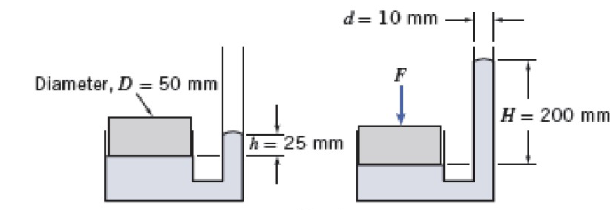
\includegraphics[width=0.5\linewidth]{./figures/e3_5.png}
  \caption{}
  \label{fig:e3_5}
\end{figure}
\bigbreak
For the system to be static the force exerted by the piston on the mercury must be equal to the force exerted by the column. When no force other than the weight of the piston itself is applied a mercury cylinder of height \qty{25}{mm} and diameter \qty{10}{mm} is produced. The height rise of this must give rise to a pressure increase given by:
\[ 
\Delta p = \rho g \Delta H
.\]
The piston must therefore supply a weight big enough to bring about this pressure. I.e.
\[ 
W = \Delta p A_p = \rho g \Delta H \cdot \pi \cdot r_p^2 = \qty{13,5}{g/cm^3} \cdot \qty{9,81}{m/s^2} \cdot \qty{25}{mm} \cdot \pi \cdot \left( \qty{25}{mm}  \right)^2 = \qty{0,26}{N} 
.\]
When the additional force is added the column rises an additional $\Delta H = \qty{175}{mm}$. Therefore we here get:
\[ 
F = \Delta p A_p = \qty{13,5}{g/cm^3} \cdot \qty{9,81}{m/s^2} \cdot \qty{175}{mm} \cdot \pi \cdot \left( \qty{25}{mm}  \right)^2 = \qty{45,5}{N} 
.\]


\exercise{3.6}
A \qty{125}{mL} cube of solid oak is held submerged by a tether as shown on \textbf{\autoref{fig:e3_6}}. Calculate the force of the water on the bottom surface of the cube and the tension in the tether.

\begin{figure} [ht]
  \centering
  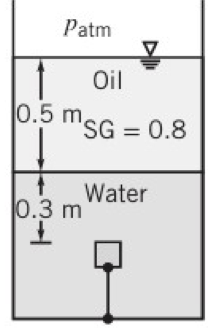
\includegraphics[width=0.25\linewidth]{./figures/e3_6.png}
  \caption{}
  \label{fig:e3_6}
\end{figure}
\bigbreak
First the side length of the cube is found as
\[ 
  s = \sqrt[3]{V_{\mathrm{oak}}} = \sqrt[3]{\qty{125}{cm^3}} = \qty{5}{cm^3} 
.\]
Now we can determine its weight as the specific gravity of oak is \num{0,77} as:
\[ 
W = V_{\mathrm{oak}} \rho \mathrm{SG}_{\mathrm{oak}} g = \qty{125}{mL} \cdot \qty{1000}{kg/m^3} \cdot \num{0,77} \cdot \qty{9,81}{m/s^2} = \qty{0,944}{N} 
.\]
The force on the bottom surface is equal to the pressure at this depth multiplied by the surface area of the bottom face. Firstly the pressure is found as:
\begin{align*}
  p_L &= p_{\mathrm{atm}} + \mathrm{SG}_{\mathrm{oil}} \cdot \rho \cdot g \cdot h_{\mathrm{oil}} + \rho g h_L \\
  &= p_{\mathrm{atm}} + \rho g \left( \mathrm{SG}_{\mathrm{oil}} \cdot h_{\mathrm{oil}} + h_L \right) \\
  &= \qty{101,325}{kPa} + \qty{1000}{kg/cm^3} \cdot \qty{9,81}{m/s^2} \left( \num{0,8} \cdot \qty{0,5}{m} + \qty{0,35}{m}  \right) \\
  &= \qty{108,6825}{kPa}  
.\end{align*}
Now this can be multiplied by the surface area of the bottom as:
\[ 
F_L = p_L \cdot A = \qty{108,6825}{kPa} \cdot \qty{25}{cm^2}  = \qty{271,7}{N} 
.\]
Therefore the force exerted by the fluid on the bottom face is about \qty{271,7}{N}.

To find the tension in the tether we realize that the force exerted by the fluid on the bottom face is counteracted by a force exerted by the fluid on the top face. We can find this using the same procedure as above.
\[ 
  F_U = \left( p_{\mathrm{atm}} + \rho g \left( \mathrm{SG}_{\mathrm{oil}} \cdot h_{\mathrm{oil}} + h_U \right) \right) \cdot A
.\]
We can calculate the resultant force exerted by the liquid on the cube as:
\[ 
\Delta F = F_L - F_U = \rho g \cdot \left( h_L - h_U \right) \cdot A = \qty{1000}{kg/m^3} \cdot \qty{9.81}{m/s^2} \cdot \left( \qty{5}{cm}  \right) \cdot \qty{25}{cm^2} = \qty{1,22625}{N}
.\]
This force (directed directly upwards) is counteracted by the weight of the cube. I.e.
\[ 
T = \Delta F - W = \qty{1,22625}{N} -\qty{0,944}{N} = \qty{0,282}{N} 
.\]



\exercise{3.43}
Determine the specific weight of the cube when one half is submerged as shown on \textbf{\autoref{fig:e3_43}}. Determine the position of the center of the cube relative to the water level when the weight is removed.

\begin{figure} [ht]
  \centering
  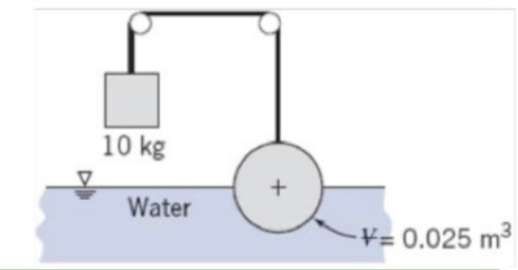
\includegraphics[width=0.5\linewidth]{./figures/e3_43.png}
  \caption{Caption}
  \label{fig:e3_43}
\end{figure}
\bigbreak
For static equilibrium the sum of the forces in the upwards/downwards direction must be 0. The only forces acting in this direction on the sphere is its weight (downwards) and the tension and the bouyancy forces (upwards). The tension in the cable must be exactly enough to keep the cube steady:
\[ 
T = M \cdot g 
.\]
The buoyancy force on the sphere is given by Archimedes principle as:
\[ 
F_B = \rho \cdot g \cdot \frac{V}{2} 
.\]
The weight of the sphere is given by:
\[ 
W = \mathrm{SG} \cdot \rho \cdot g \cdot V
.\]
These must, as mentioned, all sum to zero as:
\[ 
M g + \rho g \frac{V}{2} - \mathrm{SG} \rho g V = 0 \implies \mathrm{SG} = \frac{M}{\rho V} + \frac{1}{2}
.\]
Now known values can be substituted in as:
\[ 
\mathrm{SG} = \qty{10}{kg} \cdot \frac{1}{\qty{1000}{kg/m^3} \cdot \qty{0.025}{m^3} } + \frac{1}{2} = \num{0,9} 
.\]
The specific weight is
\[ 
\gamma = \frac{\mathrm{Weight}}{\mathrm{Volume}} = \frac{\mathrm{SG} \cdot \rho \cdot g \cdot V}{V} = \mathrm{SG} \rho \cdot g = \num{0,9}  \cdot \qty{1000}{kg/m^3} \cdot \qty{9,81}{m/s^2} = \qty{8829}{N/m^3}  
.\]

Now to find the equilibrium position when floating we repeat the force balance, but this time with $T = 0$ as
\[ 
F_B - W = 0 \implies W = F_B = \rho g V_{\mathrm{submerged}}
.\]
Now we must realize that the submerged part of the sphere will be a spherical cap. The volume of such an object is:
\[ 
V_{\mathrm{submerged}} = \frac{\pi \cdot h_{\mathrm{submerged}^2}}{3} \cdot \left( 3 \cdot R - h_{\mathrm{submerged}} \right)
.\]
Where $R$ is the radius of the sphere. The radius of the sphere can be found as:
\begin{align*}
  V &= \frac{4}{3} \pi R^3 \\
  R &= \sqrt[3]{ \frac{3V}{4\pi}} \\
    &= \sqrt[3]{\frac{3}{4\pi}\cdot \qty{0,025}{m^3} } \\
    &= \qty{0,181}{m}
.\end{align*}
Therefore:
\begin{align*}
  W &= \rho g V_{\mathrm{submerged}}\\
  \mathrm{SG} \cdot \rho g V &= \rho g \frac{\pi h_{\mathrm{submerged}^2}}{3} \cdot \left( 3 \cdot R - h_{\mathrm{submerged}} \right) \\
  \mathrm{SG} \cdot V &= \frac{\pi h_{\mathrm{submerged}^2}}{3} \left( 3 R - h_{\mathrm{submerged}}  \right) \\
  \frac{3 \mathrm{SG} \cdot V}{\pi} &= h_{\mathrm{submerged}}^2 \left( 3R - h_{\mathrm{submerged}} \right) \\
  h_{\mathrm{submerged}}^2 \left( 3 \cdot \qty{0,181}{m} - h_{\mathrm{submerged}}\right) &= \frac{3 \cdot \num{0,9} \cdot \qty{0,025}{m^3} }{\pi} \\
  h_{\mathrm{submerged}}^2 \left( \qty{0,544}{m} - h_{\mathrm{submerged}}  \right) &= \qty{0,0215}{m^3}  \\
  \implies h_{\mathrm{submerged}} &\in \{- \qty{0,173}{m}, \qty{0,292}{m}, \qty{0,425}{m} \}
.\end{align*}
Here the negative solution can be rejected as it is unphysical. The largest solution can also be rejected as $\qty{0,425}{m} > 2 \cdot R = \qty{0,362}{m}$ and this would require the sphere to be floating beneath the water surface, which is also unphysical. Therefore the sphere must be floating at a height of $h = \qty{0,292}{m}$. 
